\chapter{Resultados} \label{cap:resultados}
\vspace{-2cm}

Após as correções da simulação explicadas no Capítulo \ref{cap:simulacao} Sessão \ref{sec:bugs}, encontramos a qualidade da água $70\%$ pior do que uma água pura. Os histogramas de energia podem ser vistos nas Figuras \ref{fig:a5} e \ref{fig:b4}. A curva de transformação está representada na Figura \ref{fig:transf}.


\begin{figure*}[ht]
	\centering
	\begin{subfigure}{0.5\textwidth}
		\centering
		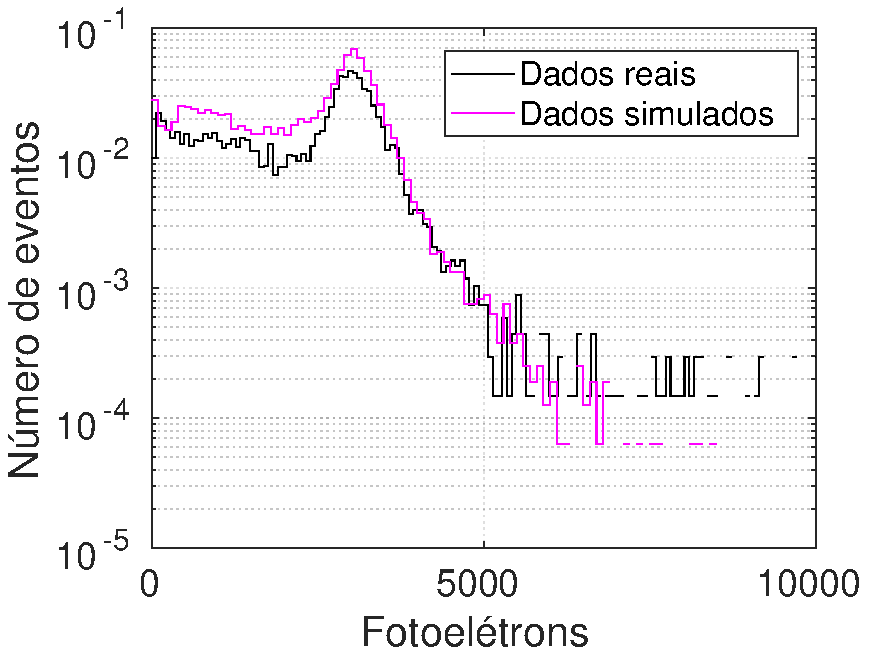
\includegraphics[width=8cm]{textuais/simulacao/figuras/hist_evt4.pdf}
		\caption{Distribuição de energia por eventos com qualidade da água 70\% pior que a original}
		\label{fig:a5}
	\end{subfigure}%
	~ 
	\begin{subfigure}{0.5\textwidth}
		\centering		
		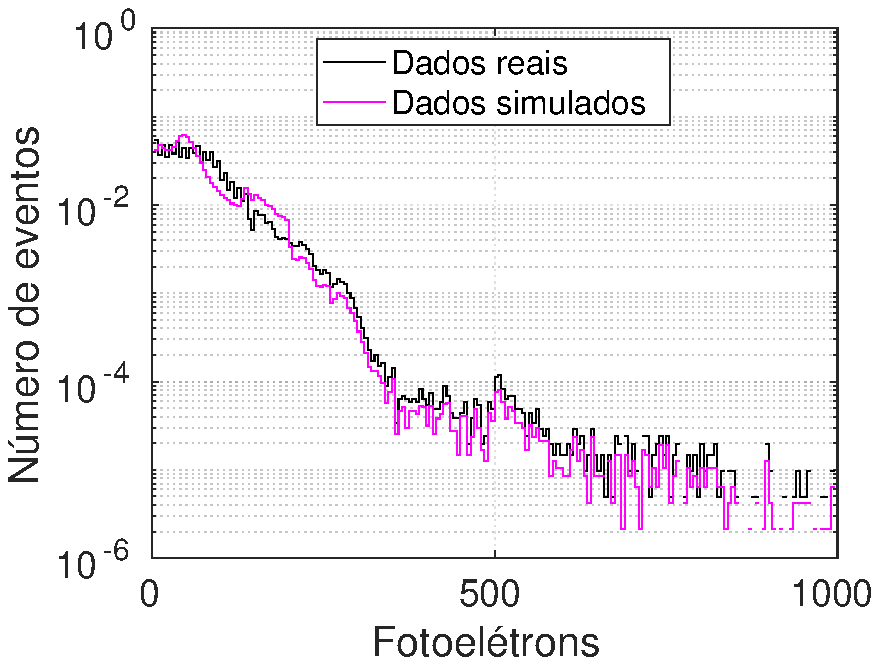
\includegraphics[width=8cm]{textuais/simulacao/figuras/hist_pmt4.pdf}
		\caption{Distribuição de energia por PMT com Qualidade da água 70\% pior que a original}
		\label{fig:b4}
	\end{subfigure}
	\caption{Comparação dos dados reais com os simulados após a transformação de CDFe modificando a qualidade da água}
\end{figure*}



\begin{figure}[H]
	\centering
	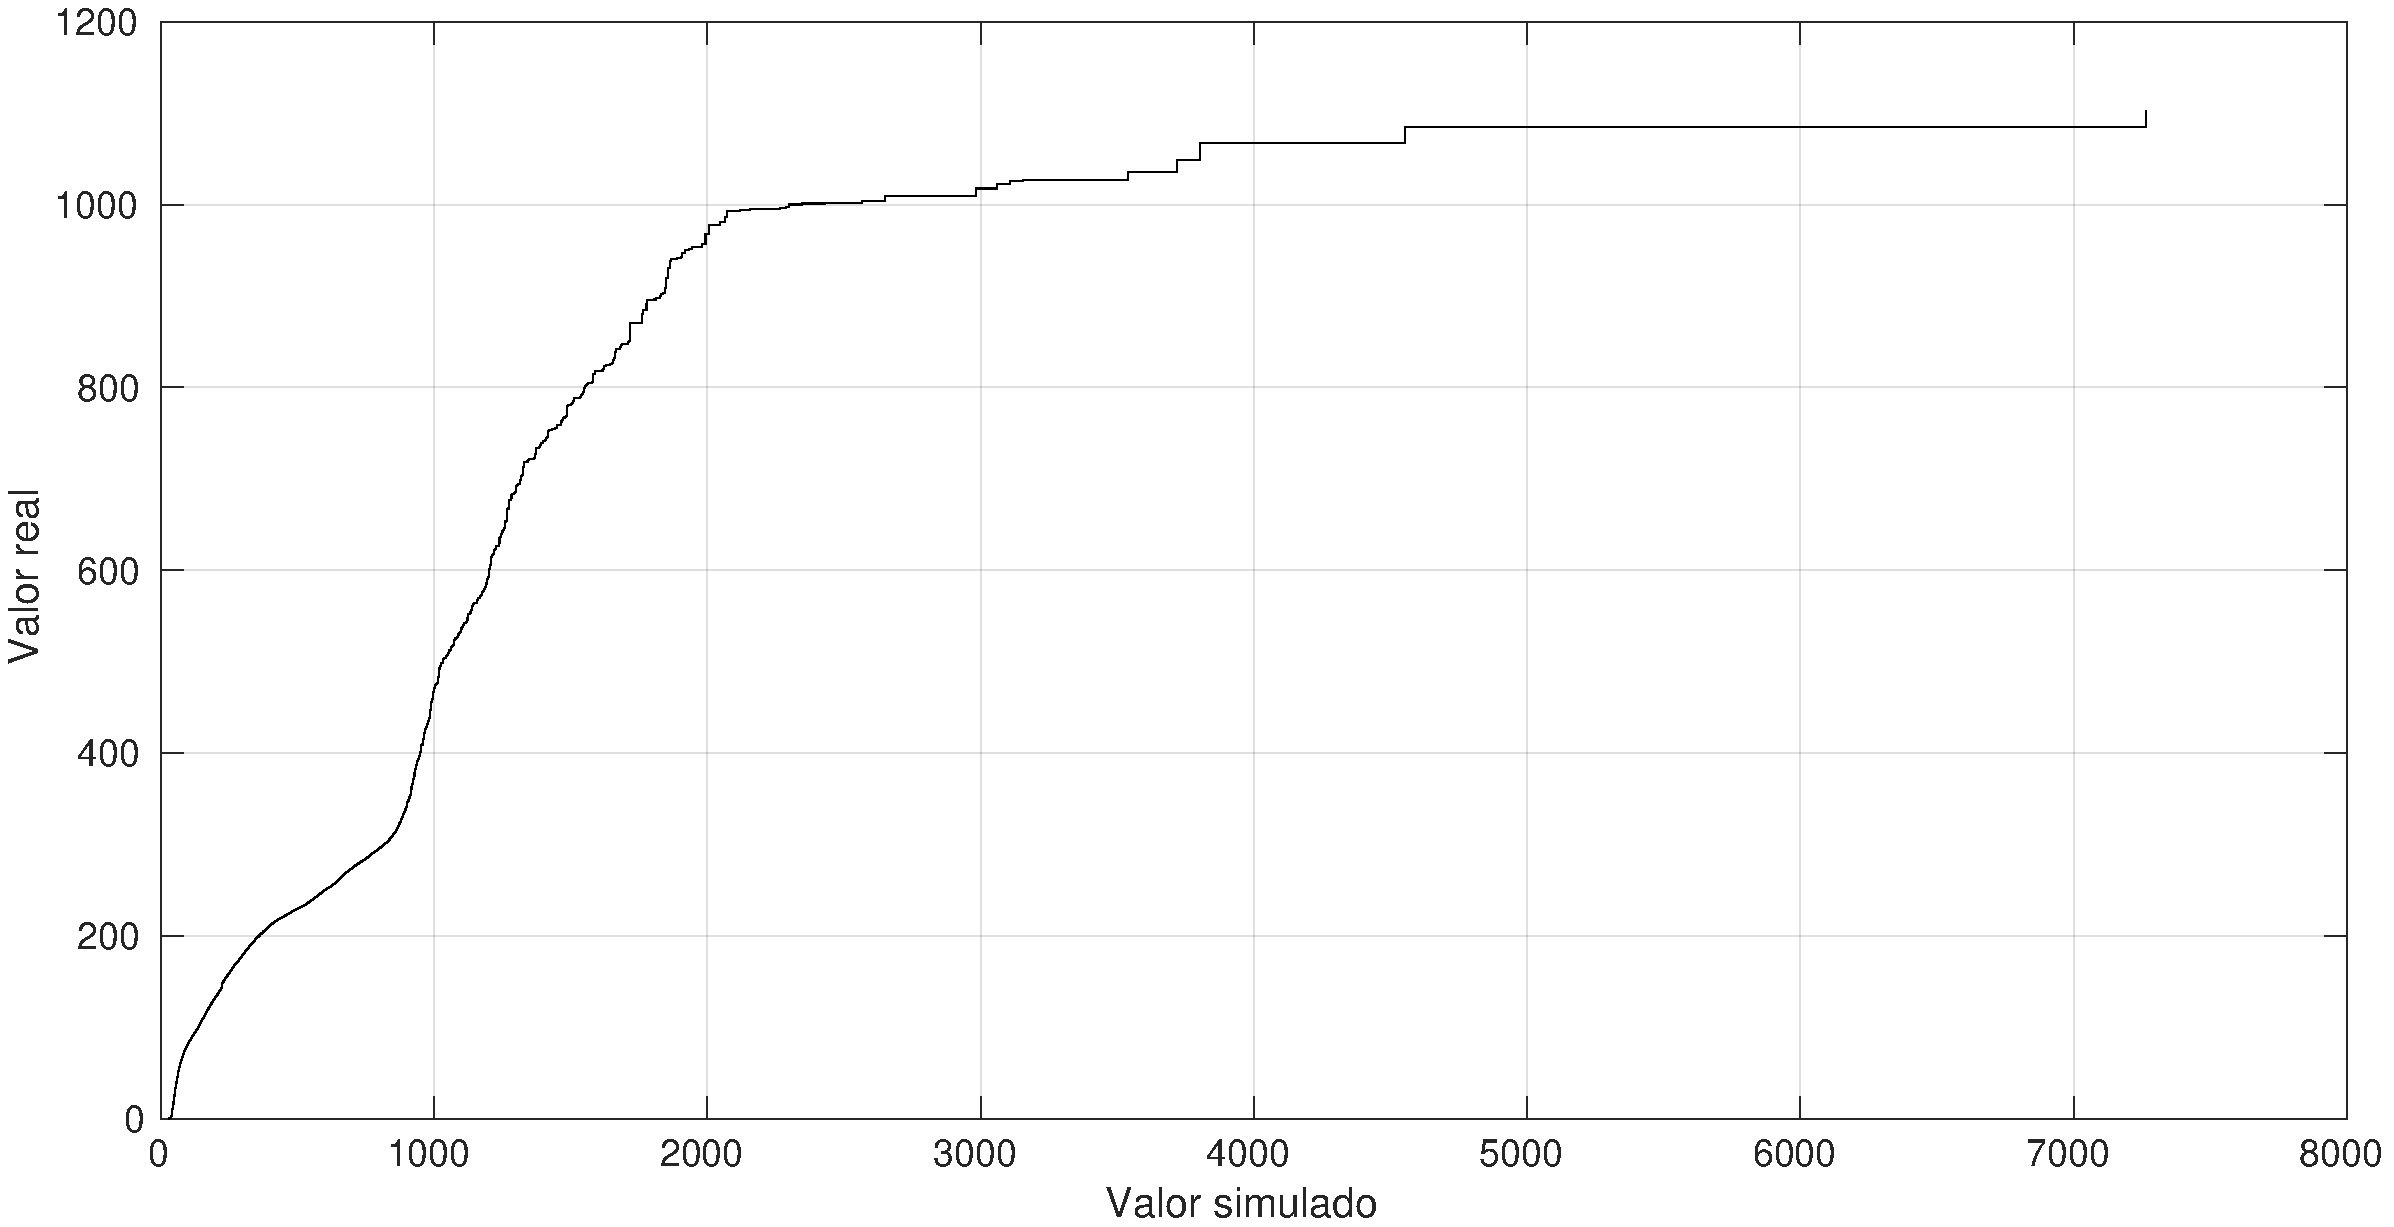
\includegraphics[width=16cm]{textuais/simulacao/figuras/transformacao.pdf}
	\caption{Transformação de CDFe dos valores simulados para valores reais }
	\label{fig:transf}
\end{figure}

Pôde ser visto uma distorção no histograma de energia por PMT (Figura \ref{fig:b4}) após o método da CDFe. Este erro pode ser atribuído à transição de transformação e os valores originais da simulação. Este problema modifica a distribuição (probabilidade) das energias porém mantém o formato da transformação.

Embora o escopo deste trabalho tenha tido foco na energia das PMTs, devemos validar a simulação através de outros métodos. Foram escolhidos o número de PMTs em coincidência por evento (multiplicidade) e a posição da PMT mais energética para esta validação.

Para a multiplicidade, observamos uma forma parecida entre os dados simulados e reais, porém com um pouco menos eventos de baixa energia, como pode ser visto comparando as Figuras \ref{fig:fired_real_comp} e \ref{fig:fired_sim_comp}. 


\begin{figure*}[ht]
	\centering
	\begin{subfigure}{0.5\textwidth}
		\centering
	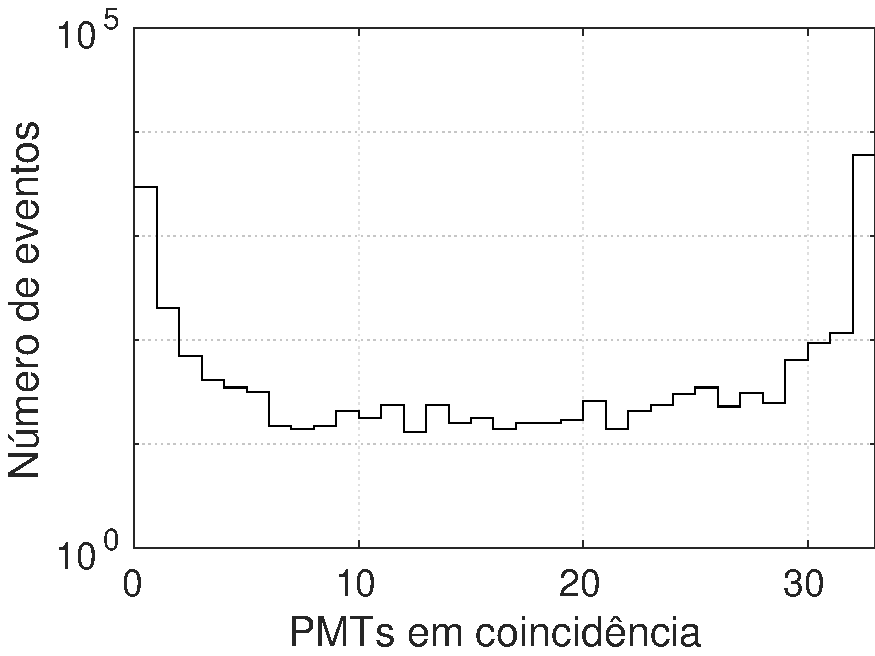
\includegraphics[width=8cm]{textuais/simulacao/figuras/firedpmt_real_comp.pdf}
		\caption{Dados adquiridos em Angra}
		\label{fig:fired_real_comp}
	\end{subfigure}%
	~ 
	\begin{subfigure}{0.5\textwidth}
		\centering
	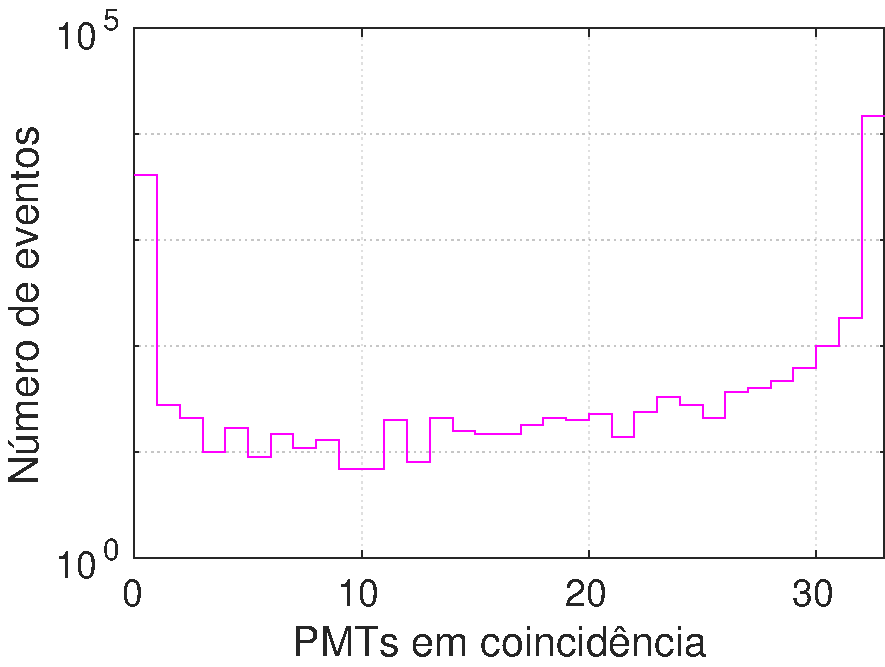
\includegraphics[width=8cm]{textuais/simulacao/figuras/firedpmt_sim_comp.pdf}
		\caption{Dados da simulação}
				\label{fig:fired_sim_comp}
	\end{subfigure}
	\caption{Comparação dos dados reais com os simulados para o número de PMTs em coincidência por evento.}
\end{figure*}

Porém, para a posição mais provável da PMT mais energética (plano inferior ou superior) tivemos uma divergência alta na região de baixas energias, enquanto que nos dados adquiridos em Angra isso não ocorreu Na simulação vemos uma grande probabilidade da PMT mais energética estar posicionada no topo para eventos de baixas energias.

Para eventos mais energéticos, o comportamento é esperado devido ao efeito Cherenkov gerado por partículas que chegam de cima para baixo, deixando mais fótons em direção às PMTs inferiores. Para os eventos de baixa energia, temos que outros eventos que não múons podem influenciar nesta região fazendo com que os dados reais não se comportem como na simulação, onde apenas múons são considerados. Mas essa e outras possíveis justificativas para esta diferença devem ser investigadas e qualquer afirmação neste momento pode ser falho.

\begin{figure*}[h]
	\centering
	\begin{subfigure}{0.5\textwidth}
		\centering
	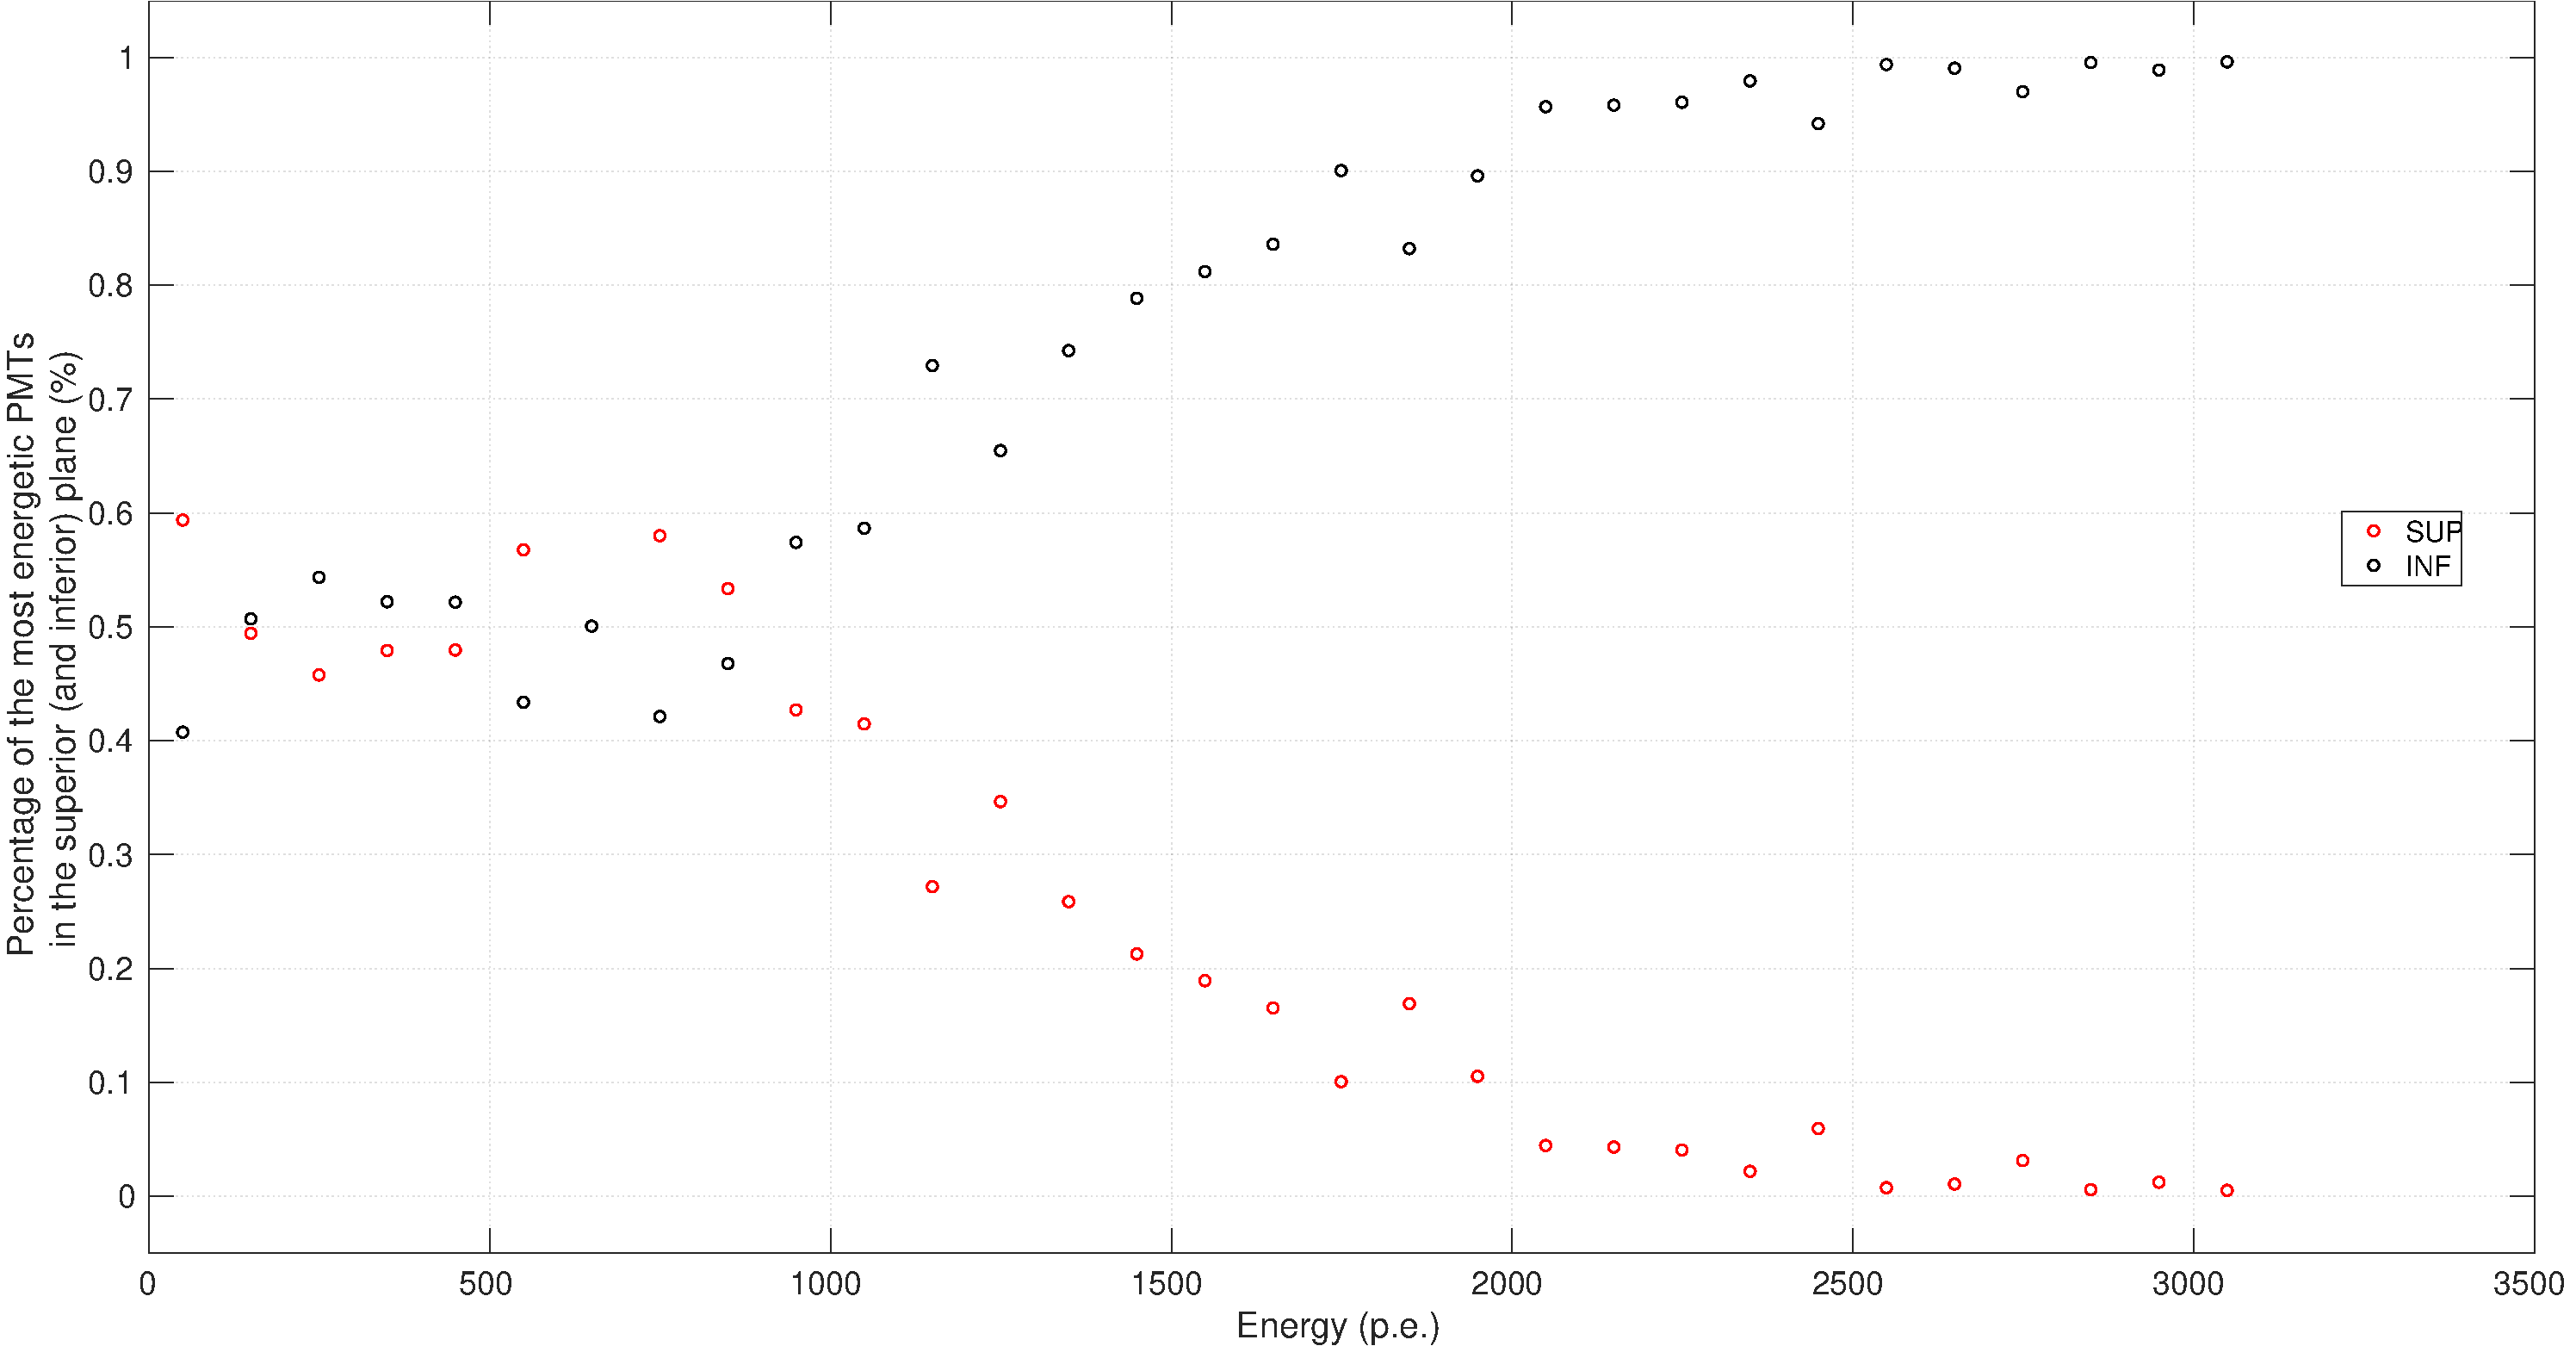
\includegraphics[width=8cm]{textuais/simulacao/figuras/probsupinf_real.pdf}
		\caption{Dados adquiridos em Angra}
		\label{fig:a}
	\end{subfigure}%
	~ 
	\begin{subfigure}{0.5\textwidth}
		\centering
	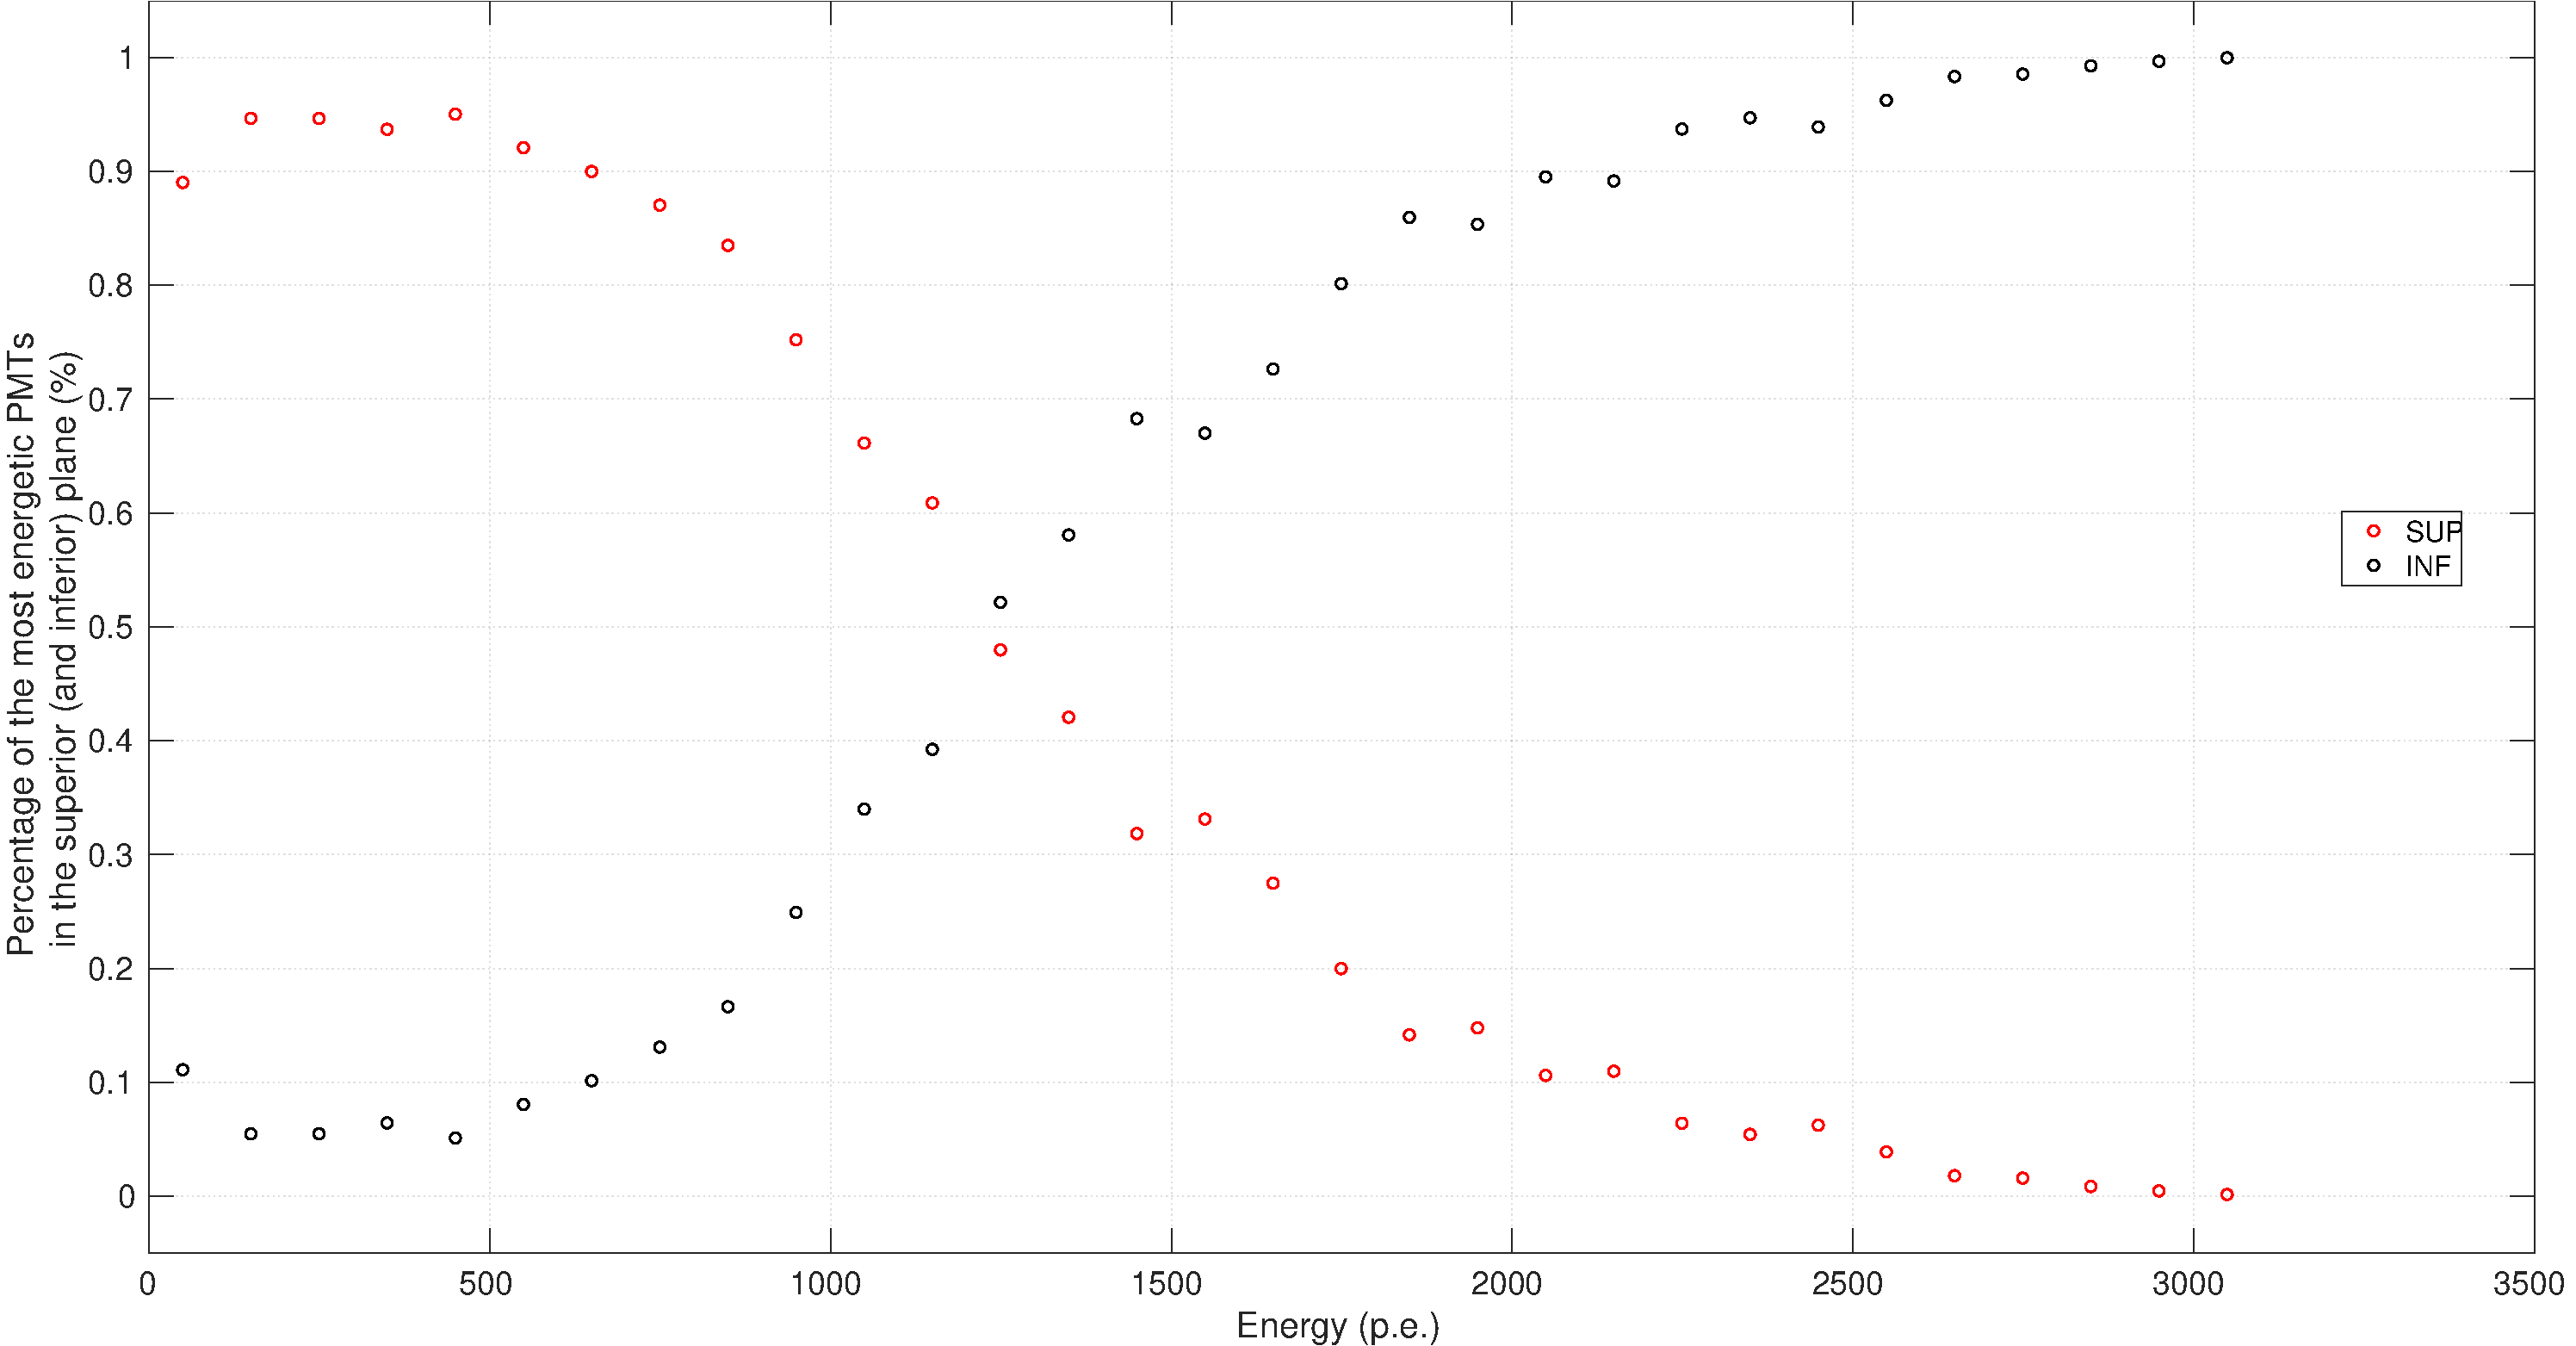
\includegraphics[width=8cm]{textuais/simulacao/figuras/probsupinf_sim.pdf}
		\caption{Dados da simulação}
				\label{fig:b}
	\end{subfigure}
	\caption{Comparação dos dados reais com os simulados para a posição da PMT mais energética por evento.}
\end{figure*}

Outros plots gerados para os dados da simulação podem ser encontrados no apêndice \ref{apdx:simulacao}.